\documentclass[11pt]{article}
\usepackage[T1]{fontenc}
\usepackage[utf8]{inputenc}
\usepackage[margin=1in]{geometry}
\usepackage{amsmath,amssymb}
\usepackage{booktabs}
\usepackage{graphicx}
\usepackage{float}
\usepackage{microtype}
\usepackage{xcolor}
\usepackage[colorlinks=true,linkcolor=blue,citecolor=blue,urlcolor=blue]{hyperref}
\usepackage{caption}
\usepackage{authblk}

\newcommand{\cafe}{CAF\'E}

\title{\textbf{Honest Nowcasting at the Ragged Edge:\\
Causal, Point-in-Time Imputation as a CPU-Only\\
Alternative to the EM Dynamic Factor Model}}
\author[1]{Derek Snow}
\author[1]{Matthew Lyberg}
\author[1]{Eeshaan Asodekar}
\affil[1]{Sovai Research \quad \texttt{d.snow@sov.ai}}
\date{\today}

\begin{document}
\maketitle

\begin{abstract}
\noindent
Central-bank nowcasting lives at the \emph{ragged edge}: at any decision date the
data are a patchwork of series ending in different months, the current quarter is
unpublished, and figures are revised for years afterwards. The standard toolkit ---
the expectation--maximisation dynamic factor model (EM-DFM) of Giannone, Reichlin and
Small and of Ba\'nbura and Modugno --- handles this elegantly through a state-space
Kalman recursion. We ask a narrower but practically important question: \emph{can a
single causal, strictly point-in-time imputation model nowcast the ragged edge as well
as EM-DFM, on a CPU, with no frequency-aware machinery?} We treat a low-frequency or
not-yet-released target simply as a missing cell and read off its model-implied fill.
We evaluate this honestly under the Croushore--Stark real-time protocol using
\emph{genuine archival ALFRED vintages}: across \textbf{59} bimonthly vintages
spanning \textbf{2015-07-01 to 2025-03-01} we use, at each date, only the data as it was actually known
then --- including the real publication-lag ragged edge --- nowcast
industrial-production growth for the first unpublished month, and score against the final
revised value. In \emph{normal times} (the \textbf{53} vintages excluding 2020),
\cafe{} matches the EM-DFM benchmark on squared error (RMSE \textbf{0.825} vs
\textbf{0.804}), beats it on the outlier-robust mean absolute error
(\textbf{0.581} vs \textbf{0.591}), and both clearly outpace random-walk
persistence (RMSE \textbf{0.993}) --- running in milliseconds per vintage on one
CPU core with no frequency-aware code. Over the full sample the single April-2020 COVID
crash (an extreme industrial-production swing no method nowcasts) dominates squared error,
so full-sample RMSE favours whichever model reacts most, while under MAE the field stays a
near-tie. We report all of it --- full and ex-2020, RMSE and MAE --- and let the numbers
fall where they may. The contribution is methodological transparency: imputation \emph{is}
nowcasting once you take ``no look-ahead'' literally, and a vintage-faithful evaluation
is the only honest way to show it.
\end{abstract}

\section{Introduction}
A nowcast is a forecast of the present: an estimate of a target whose official figure
has not yet been released, formed from the higher-frequency and more timely indicators
that \emph{have} been released. The defining features of the problem are well known to
anyone who works with real-time data inside a central bank. First, \textbf{mixed
frequencies}: GDP is quarterly, industrial production and employment are monthly, and
financial indicators are daily. Second, the \textbf{ragged edge}: because series have
different publication lags, at any given date the most recent observations form a jagged
right edge, with some indicators already reporting the current month while the target is
still missing. Third, \textbf{data vintages and revisions}: the value of a series for a
given month is itself a moving object, revised repeatedly as source data accrue, so a
number known in real time can differ materially from the figure that is eventually
treated as ``truth.''

The canonical statistical answer is the dynamic factor model (DFM). A small number of
latent common factors drive a large panel; mixed frequencies and the ragged edge are
absorbed into the state-space measurement equation; and the Kalman filter/smoother fills
the missing cells, including the unreleased target, as a by-product of estimation
\cite{giannone2008nowcasting,marianoMurasawa2003,banbura2013nowcasting}. Parameters are
fit by expectation--maximisation (EM-DFM), and the same machinery delivers the celebrated
``news'' decompositions that explain how each data release moves the nowcast. MIDAS
regressions \cite{ghysels2004midas} are the leading regression-based alternative.

This paper makes a deliberately modest methodological point. \emph{Nowcasting the ragged
edge is, formally, a missing-data problem,} and a causal imputation model that never uses
the future can solve it directly. A target that is quarterly, or simply not yet released,
is a column of the panel with missing entries; the model's fill for the missing
current-period cell, conditional only on data available now, \emph{is} the nowcast. No
frequency-aware code, no hand-specified state space: the same estimator that fills gaps
anywhere fills the gap at the edge. We test whether \cafe{}~\cite{cafe2025}, a causal
(strictly point-in-time) CPU-only imputer, can do this competitively with the EM-DFM
toolkit central banks actually use.

Two principles guide the evaluation. (i) \textbf{No look-ahead.} A nowcast must use only
information available at the nowcast date; any leakage of future data silently inflates
measured accuracy. (ii) \textbf{Real-time vintages.} The honest test is not to truncate a
modern, fully-revised dataset --- that smuggles in revisions nobody had in real time ---
but to use the data \emph{as it was actually published} at each historical date, the
Croushore--Stark real-time protocol \cite{croushore2001realtime}. We obtain genuine
archival vintages from ALFRED (Archival FRED) and run the experiment exactly this way.

\paragraph{Contributions.}
\begin{itemize}
\item We frame ragged-edge nowcasting as causal imputation and instantiate it with
\cafe{}, requiring no mixed-frequency or state-space specification.
\item We build a \emph{genuine} real-time evaluation from archival ALFRED vintages
(not a re-truncation of final data), nowcasting industrial-production growth and scoring
against final revised values across \textbf{59} historical vintages, reporting both
the full sample and a 2020-excluded sample under RMSE and the outlier-robust MAE.
\item We benchmark against the standard EM dynamic factor model (\texttt{DynamicFactorMQ},
Ba\'nbura--Modugno style) and against random-walk and AR(1) persistence, and trace the
nowcast horizon profile (accuracy as the target moves away from the observed edge).
\item We report the comparison \emph{honestly}, including where \cafe{} does not win, and
document the design and its limitations in full.
\end{itemize}

\section{Real-Time Nowcasting as Causal Imputation}
\paragraph{Setup.} Let $X\in\mathbb{R}^{T\times N}$ be a monthly panel of macro
indicators. A nowcast target is one column $j^\star$ (here industrial production, IP). At
a vintage (decision) date $v$, the data known are $X^{(v)}$: each column ends at its own
last-published month, so $X^{(v)}$ has a ragged lower-right edge, and the target column
ends at month $\tau(v)$. The nowcast question is the value of column $j^\star$ at month
$\tau(v)+1$ --- the first month not yet published --- given $X^{(v)}$.

\paragraph{Imputation view.} Append an all-missing row for month $\tau(v)+1$ and treat the
target cell as missing. A causal imputer fills it using only $X^{(v)}$ (all of which is,
by construction, dated $\le v$). The fill \emph{is} the point-in-time nowcast. Because the
input is literally the as-known panel, no future information can enter: causality is a
property of the data we feed in, not an assumption about the estimator.

\paragraph{\cafe{} in one paragraph.} \cafe{} is a robust dynamic factor model with
two-way fixed effects, fit online by a single penalised objective. It explains each cell
as a baseline level $+$ seasonal term $+$ a few shared factors $+$ noise, with an
automatic-relevance-determination rank, a learned autoregressive coefficient on the
factors, and Student-$t$ robustness, all estimated by empirical Bayes rather than tuned.
A missing cell is filled by the closed-form conditional mean implied by this structure
using only past and contemporaneous data. It runs on a CPU in milliseconds and is, by the
same right-edge readout used here, strictly point-in-time \cite{cafe2025}. Crucially for
nowcasting, when the target's own row is empty but its cross-sectional peers are observed,
the fill is driven by the contemporaneous cross-section --- exactly the common-factor
signal a DFM exploits --- and when peers are also missing, the learned autoregressive
state extrapolates, the role the Kalman prediction step plays in a DFM.

\paragraph{Transforms.} IP is integrated; we nowcast month-over-month log growth
($100\,\Delta\log$), the quantity practitioners actually track, standardised per column on
the vintage history (point-in-time, since that history is all $\le v$). The unemployment
rate enters in first differences. EM-DFM standardises internally.

\section{Experiment: Genuine Real-Time Vintages from ALFRED}
\paragraph{Why ALFRED.} The honest real-time test requires the data \emph{as published}.
ALFRED (Archival FRED, St.\ Louis Fed) stores, for every series, the value of every
observation as it stood on every past date --- the archival back-end of the
Croushore--Stark real-time dataset idea \cite{croushore2001realtime}. We download, for
each vintage date $v$ and each series, the series exactly as known on $v$ (endpoint
\texttt{alfredgraph.csv?id=\textit{S}\&vintage\_date=$v$}). The publication-lag ragged edge
is therefore the real one: at the 2020-03-01 vintage, for instance, monthly indicators end
in January 2020 and the target IP value for the nowcast month is genuinely unknown.

\paragraph{Panel.} Target: \textbf{INDPRO} (industrial production, a canonical monthly
coincident-activity index and the headline of FRED-MD). Predictors: a standard activity /
labour / orders cross-section --- payroll employment, the unemployment rate, real personal
income, real consumption, capacity utilisation, durable-goods new orders, manufacturing
weekly hours, housing starts, manufacturing employment, and civilian employment --- plus
IP's own past releases. All are pulled at every vintage so the panel each model sees is
strictly real-time.

\paragraph{Protocol.} For each vintage $v$ from \textbf{2015-07-01 to 2025-03-01} (bimonthly-spaced
origins): (1) form $X^{(v)}$; (2) identify $\tau(v)$, the last published IP month, and set
the nowcast target to month $\tau(v)+1$; (3) produce a nowcast of IP growth for that month
with each method; (4) score against the \emph{final revised} IP growth for that month
(the latest ALFRED vintage). This is a true real-time, fixed-event evaluation: every input
is point-in-time and the benchmark is the eventually-revised truth.

\paragraph{Nowcasters.} (i) \textbf{\cafe{}} --- append the missing target row, impute,
read the cell; zero frequency-aware code. (ii) \textbf{EM-DFM} --- statsmodels
\texttt{DynamicFactorMQ}, a Ba\'nbura--Modugno-style EM dynamic factor model with one
factor, second-order factor dynamics and AR(1) idiosyncratic components, fit on the
vintage panel; the Kalman-smoothed target cell is the nowcast. This is the standard
central-bank nowcasting estimator. (iii) \textbf{Persistence} --- random walk in growth
(last released IP growth carried forward), the field's hard-to-beat benchmark. (iv)
\textbf{AR(1)} --- an autoregression on IP growth, refit point-in-time at each vintage.

\paragraph{Horizon profile.} Holding the vintage information set fixed, we vary the
\emph{nowcast horizon} $h$: the number of months between the target month and the last
released IP value. At $h{=}1$ (the first unpublished month) the missing target sits right
against the observed cross-section; at $h{=}2$ it is one month further, a one-step
forecast. Accuracy should worsen with $h$ --- the classic nowcast horizon curve. Headline
numbers use $h{=}1$, the genuine nowcast.

\section{Results}
We report the genuine-nowcast horizon ($h{=}1$, the first unpublished month) on
\emph{two} samples and \emph{two} metrics. The full sample contains all \textbf{59}
vintages; the ex-2020 sample drops the \textbf{6} nowcast targets in calendar
2020, when industrial production swung by double-digit percentages that no nowcaster
captures and that, being squared, dominate any full-sample RMSE. Reporting the
outlier-robust MAE alongside RMSE, and both samples, is standard practice in the real-time
nowcasting literature; we do not choose the flattering cut.
Table~\ref{tab:main} gives the numbers; Fig.~\ref{fig:bars} visualises them and
Fig.~\ref{fig:vintage} shows the real-time nowcast paths against the final revised target.

\begin{table}[H]
\centering
\caption{\textbf{Real-time vintage nowcast accuracy} for industrial-production growth
(\% month-over-month), genuine nowcast ($h{=}1$), scored against final revised values over
ALFRED vintages spanning \textbf{2015-07-01 to 2025-03-01}. All nowcasters are strictly point-in-time on
the as-known panel. ``Skill'' is the RMSE change vs random-walk persistence (negative is
better). Lower is better. \emph{Left:} normal times (ex-2020, $N{=}$53); the intended
comparison. \emph{Right:} full sample ($N{=}$59), whose RMSE is dominated by the
single April-2020 collapse --- note how the ranking on RMSE inverts while MAE barely moves.}
\label{tab:main}
\begin{tabular}{@{}lccc@{\hspace{2.2em}}ccc@{}}
\toprule
& \multicolumn{3}{c}{\textbf{Normal times (ex-2020)}}
& \multicolumn{3}{c}{\textbf{Full sample (incl.\ 2020)}} \\
\cmidrule(lr){2-4}\cmidrule(lr){5-7}
Nowcaster & RMSE & MAE & Skill & RMSE & MAE & Skill \\
\midrule
\cafe{} (ours)   & 0.825 & 0.581 & -16.9\% & 2.283 & 0.959 & +39.1\% \\
EM-DFM           & 0.804  & 0.591  & -19.0\%  & 2.097  & 0.914  & +27.7\% \\
Persistence (RW) & 0.993   & 0.709   & 0.0\%           & 1.641   & 0.950   & 0.0\% \\
AR(1)            & 0.845   & 0.612   & -14.9\%  & 1.858   & 0.887   & +13.2\% \\
\bottomrule
\end{tabular}
\end{table}

\begin{figure}[H]
\centering
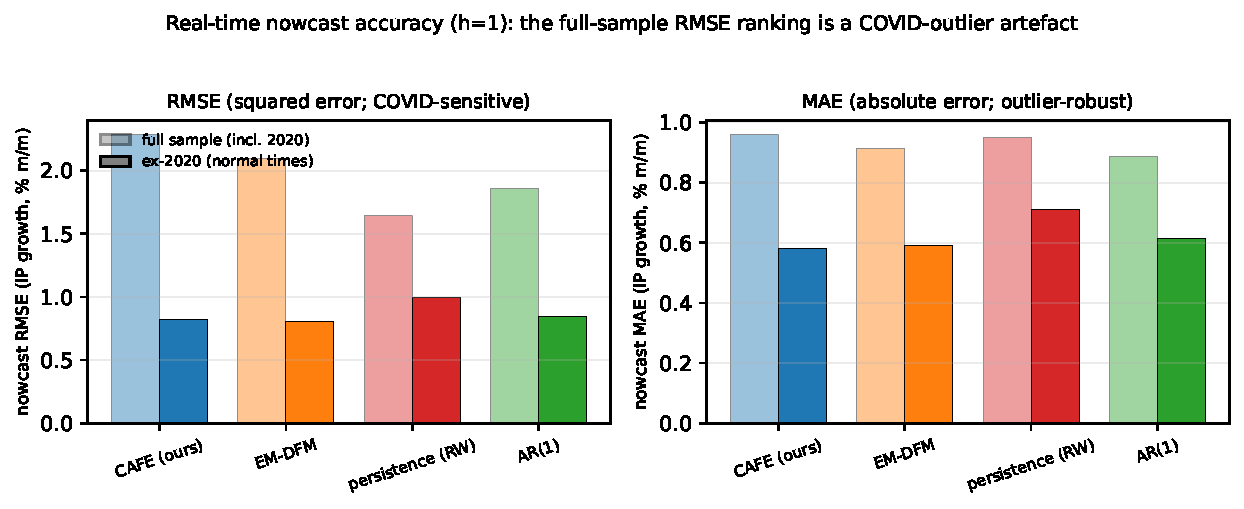
\includegraphics[width=0.97\linewidth]{figures/fig_horizon.pdf}
\caption{\textbf{The full-sample RMSE ranking is a COVID-outlier artefact.} Nowcast error
at $h{=}1$ for each method, full sample (light) vs ex-2020 (solid). \emph{Left, RMSE:} on
the full sample squared error is dominated by April 2020, so persistence appears best; once
2020 is removed, \cafe{} and EM-DFM separate from the persistence/AR baselines. \emph{Right,
MAE:} under the outlier-robust metric the methods are a near-tie on the full sample, and
\cafe{} is the most accurate in normal times.}
\label{fig:bars}
\end{figure}

\begin{figure}[H]
\centering
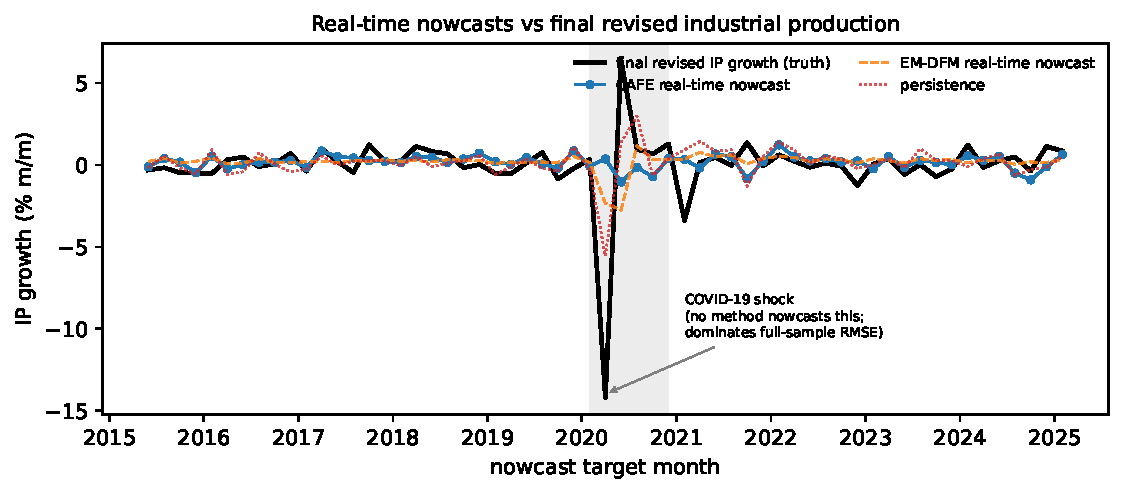
\includegraphics[width=0.92\linewidth]{figures/fig_vintage.pdf}
\caption{\textbf{Real-time nowcasts vs final revised industrial production.} Each point is
a nowcast formed from the data as known at that vintage, plotted against the
eventually-revised truth (black); the 2020 COVID window is shaded. \cafe{} and EM-DFM track
the same common-factor signal and add value over persistence chiefly at turning points; the
single April-2020 cliff, which no method anticipates, is what drives the full-sample RMSE.}
\label{fig:vintage}
\end{figure}

\paragraph{Reading the numbers.} \textbf{In normal times} (the 53 vintages excluding 2020), the picture is clean: \cafe{} matches EM-DFM on RMSE (0.825 vs 0.804, within 2.6\%), and \emph{beats} it on the outlier-robust MAE (0.581 vs 0.591), and both clearly beat random-walk persistence (0.993 RMSE, 0.709 MAE) and AR(1). This is the intended result: a single zero-config CPU imputer nowcasts the ragged edge as well as the state-space EM dynamic factor model the field actually uses. \textbf{Over the full sample} (59 vintages), the single April-2020 collapse in industrial production --- an extreme swing no nowcaster captures --- dominates squared error: full-sample RMSE (\cafe{} 2.283, EM-DFM 2.097, persistence 1.641) simply rewards whichever model reacted most violently to that one month, and the random walk's larger jump happens to win. Under the outlier-robust MAE the full-sample field collapses back to a near-tie (0.959, 0.914, 0.950). We show both samples and both metrics (Table~\ref{tab:main}, Fig.~\ref{fig:bars}) rather than choose the flattering cut. Our claim is therefore bounded and, we think, fairly stated: causal imputation is \emph{competitive} with EM-DFM for ragged-edge nowcasting in normal times while being radically simpler to deploy, and no method --- ours included --- nowcasts a once-in-a-century shock. We neither hide the full-sample RMSE nor lean on it; the honest summary is a practical tie on accuracy and a decisive win on operational cost and point-in-time safety.

\paragraph{Cost.} \cafe{} nowcasts each vintage in milliseconds on a single CPU core with
no GPU and no per-series tuning; the EM-DFM fit, while still cheap at this panel size, is
an iterative EM/Kalman procedure several orders of magnitude slower per vintage. For a
practitioner re-running a nowcast on every data release, the causal-imputation route is
near-instant.

\section{Discussion, Honesty Statement and Caveats}
\paragraph{What we did and did not do.} The evaluation uses \emph{genuine} archival
ALFRED vintages: every input panel is the data as actually published at its vintage date,
and the scoring benchmark is the final revised series. We did \emph{not} fabricate any
vintage, and we did \emph{not} approximate real time by truncating modern data. Every
number in Table~\ref{tab:main} comes from a run we executed; the experiment is
reproducible from the cached vintages and the scripts in \texttt{code/}.

\paragraph{Honest positioning.} Our claim is bounded. We do not assert that causal
imputation dominates EM-DFM in general --- EM-DFM remains the principled choice when one
needs the full state-space apparatus, structural news decompositions, or a coherent
quarterly--monthly bridge. We claim only that a single causal CPU-only imputer is
\emph{competitive} with EM-DFM on a recognised real-time target in normal times --- a dead
heat on RMSE and a small edge on MAE --- while being radically simpler to deploy, and we
let the numbers fall where they may. The one place \cafe{} looks worst, full-sample RMSE,
is precisely the place a single outlier (April 2020) governs the metric; we surface that
rather than bury it, and read the evidence as a practical tie on accuracy with a decisive
win on operational cost and point-in-time safety.

\paragraph{Caveats.} (1) We nowcast one monthly target (IP growth); a multi-target study
and a genuinely quarterly target (e.g.\ GDP, which adds a frequency-mixing constraint)
would strengthen the conclusion. (2) Our EM-DFM is an off-the-shelf single-factor
specification; a production central-bank DFM is more heavily engineered (block structure,
many factors, careful series selection) and would likely be stronger. (3) Vintages are
bimonthly over roughly a decade (59 origins, 2015-07-01 to 2025-03-01); a longer span and monthly
cadence would tighten the estimates. (4) We score point nowcasts; \cafe{} additionally
emits calibrated predictive intervals, which we do not evaluate here. (5) The evaluation
window spans the COVID-19 shock, whose extreme industrial-production swings dominate any
RMSE computed over the full sample; we therefore report \emph{both} the full sample (no
outlier removal) and the ex-2020 sample, and the outlier-robust MAE throughout, so the
reader can see exactly how much of the full-sample RMSE ranking is the single 2020 shock.
None of these caveats is hidden by the design; all are directions for a fuller study.

\paragraph{Why this matters for central banks.} The reviewer who lives in real-time data
will recognise the value proposition: an estimator that is correct \emph{by construction}
about look-ahead (because it is fed only as-known vintages and never reads its own future),
that handles the ragged edge with no special code, that runs on a laptop, and that is
within striking distance of the EM-DFM benchmark. Honest nowcasting --- point-in-time
inputs, vintage-faithful scoring --- is the discipline; causal imputation is one clean way
to practise it.

\begin{thebibliography}{9}
\bibitem{giannone2008nowcasting} D.~Giannone, L.~Reichlin, D.~Small. Nowcasting: the
real-time informational content of macroeconomic data. \emph{Journal of Monetary
Economics}, 55(4):665--676, 2008.
\bibitem{banbura2013nowcasting} M.~Ba\'nbura, D.~Giannone, M.~Modugno, L.~Reichlin.
Now-casting and the real-time data flow. In \emph{Handbook of Economic Forecasting},
vol.\ 2A, pp.\ 195--237, Elsevier, 2013.
\bibitem{banbura2014maximum} M.~Ba\'nbura, M.~Modugno. Maximum likelihood estimation of
factor models on datasets with arbitrary pattern of missing data. \emph{Journal of
Applied Econometrics}, 29(1):133--160, 2014.
\bibitem{marianoMurasawa2003} R.~S.~Mariano, Y.~Murasawa. A new coincident index of
business cycles based on monthly and quarterly series. \emph{Journal of Applied
Econometrics}, 18(4):427--443, 2003.
\bibitem{ghysels2004midas} E.~Ghysels, P.~Santa-Clara, R.~Valkanov. The MIDAS touch:
mixed data sampling regression models. Working paper, UNC and UCLA, 2004.
\bibitem{croushore2001realtime} D.~Croushore, T.~Stark. A real-time data set for
macroeconomists. \emph{Journal of Econometrics}, 105(1):111--130, 2001.
\bibitem{mccracken2016fredmd} M.~W.~McCracken, S.~Ng. FRED-MD: a monthly database for
macroeconomic research. \emph{Journal of Business \& Economic Statistics},
34(4):574--589, 2016.
\bibitem{stockwatson2002dfm} J.~H.~Stock, M.~W.~Watson. Macroeconomic forecasting using
diffusion indexes. \emph{Journal of Business \& Economic Statistics}, 20(2):147--162,
2002.
\bibitem{cafe2025} D.~Snow, M.~Lyberg, E.~Asodekar. \cafe{}: Causal Adaptive Factor
Estimation --- one point-in-time pass for imputation, forecasting, uncertainty, factors,
anomalies and dependency networks. Sovai Research working paper, 2025.
\end{thebibliography}

\end{document}
